\section{Scenario 2 Action-Mode Scalability Evaluation (1h, 10 Hz)}
\label{sec:scen2_sweep}

This section evaluates tactical-resolution scalability in Scenario 2 by comparing one baseline mode (\texttt{no\_daidalus\_python2}) against three DAIDALUS action modes (\texttt{safe\_band}, \texttt{preferred\_horizontal\_resolution}, and \texttt{discrete\_action}).
The experiment uses fixed simulation conditions: 1 hour virtual time (\texttt{duration\_s=3600}), \texttt{physics\_hz=10}, fixed seed (\texttt{42}), and fleet sizes $N \in \{50,100,200,500,1000\}$ for the plots and discussion below (larger $N$ sweeps may exist separately).

\subsection{Dataset status}

The run directory
\texttt{experiments/xtm\_primordial\_rust/results/scen2\_daidalus\_sweep/run\_20260324\_210239Z}
contains a complete four-variant grid for each $N$ listed above.
Figures were generated with \texttt{documentation/report\_sections/figures/scen2\_daidalus\_sweep/build\_figures.py} (\texttt{--max-n 1000}), reading per-cell \texttt{sim\_metrics.json} / \texttt{sweep\_cell.json} under \texttt{runs/}.

\subsection{Key outcomes}

\begin{table}[htbp]
\caption{Representative values at $N=1000$}
\label{tab:scen2_n1000}
\begin{center}
\begin{tabular}{|l|r|r|r|r|}
\hline
\textbf{Variant} & \textbf{Completion} & \textbf{MACproxy} & \textbf{Ineff.\%} & \textbf{Wall s} \\
\hline
no\_daidalus\_python2 & 0.4602 & 3601  & 145.56 & 155.49 \\
daidalus\_safe\_band   & 0.3344 & 19050 & 138.48 & 14721.01 \\
daidalus\_preferred\_horizontal\_resolution & 0.3063 & 1202 & 90.85 & 11447.87 \\
daidalus\_discrete\_action & 0.8079 & 3132 & 17.89 & 2235.18 \\
\hline
\end{tabular}
\end{center}
\end{table}

\noindent Across high-density cases ($N=500$ and $N=1000$), \texttt{discrete\_action} is the strongest trade-off:
higher mission completion, much lower route inefficiency, and lower alert pressure than other DAIDALUS action modes.
\texttt{safe\_band} and \texttt{preferred\_horizontal\_resolution} show severe wall-time growth at high $N$.

\subsection{Figures}

The following charts use the same sweep run and exclude any $N>1000$ so all series are comparable across variants.

\begin{figure}[htbp]
\centerline{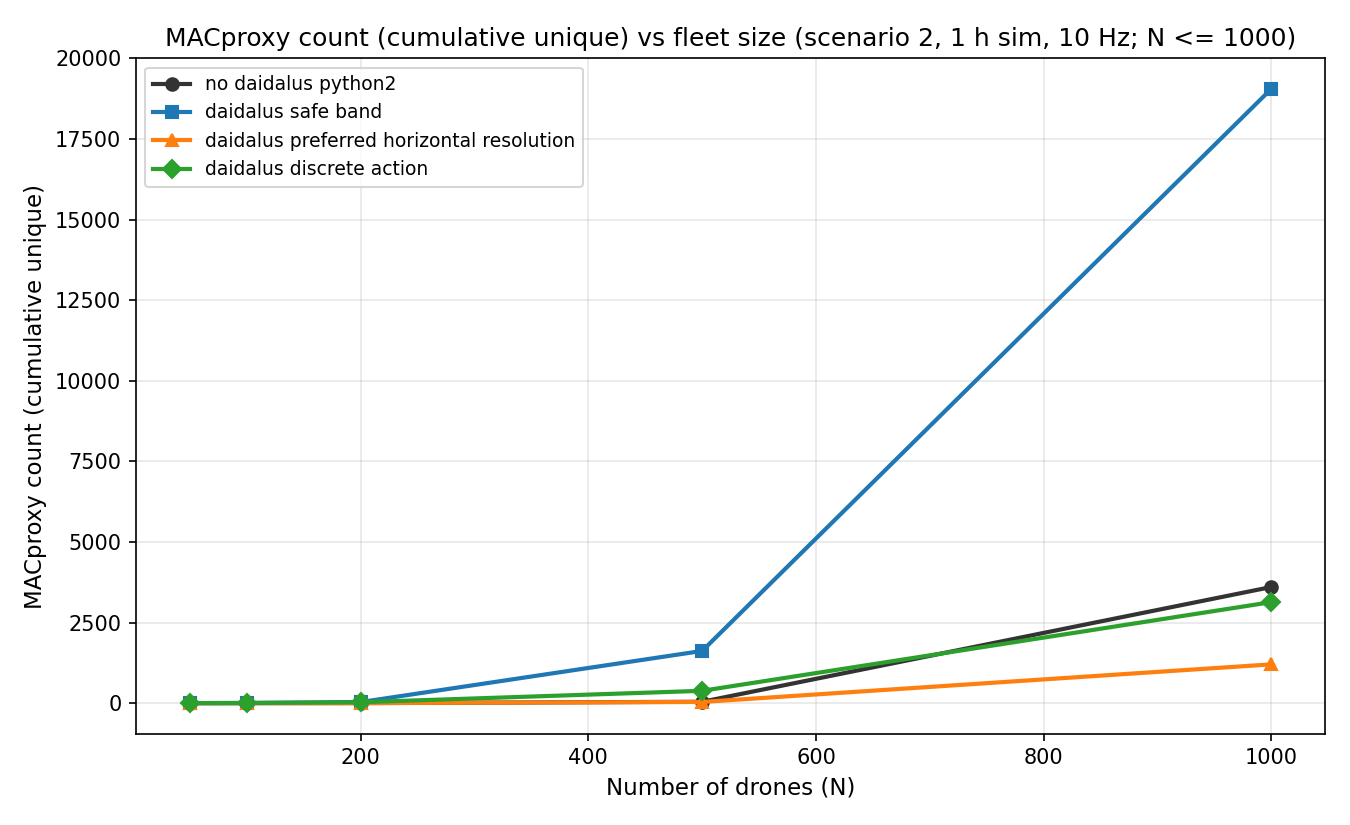
\includegraphics[width=\linewidth]{documentation/report_sections/figures/scen2_daidalus_sweep/fig_scen2_macproxy_vs_n.png}}
\caption{MACproxy count vs fleet size.}
\label{fig:scen2_macproxy}
\end{figure}

\begin{figure}[htbp]
\centerline{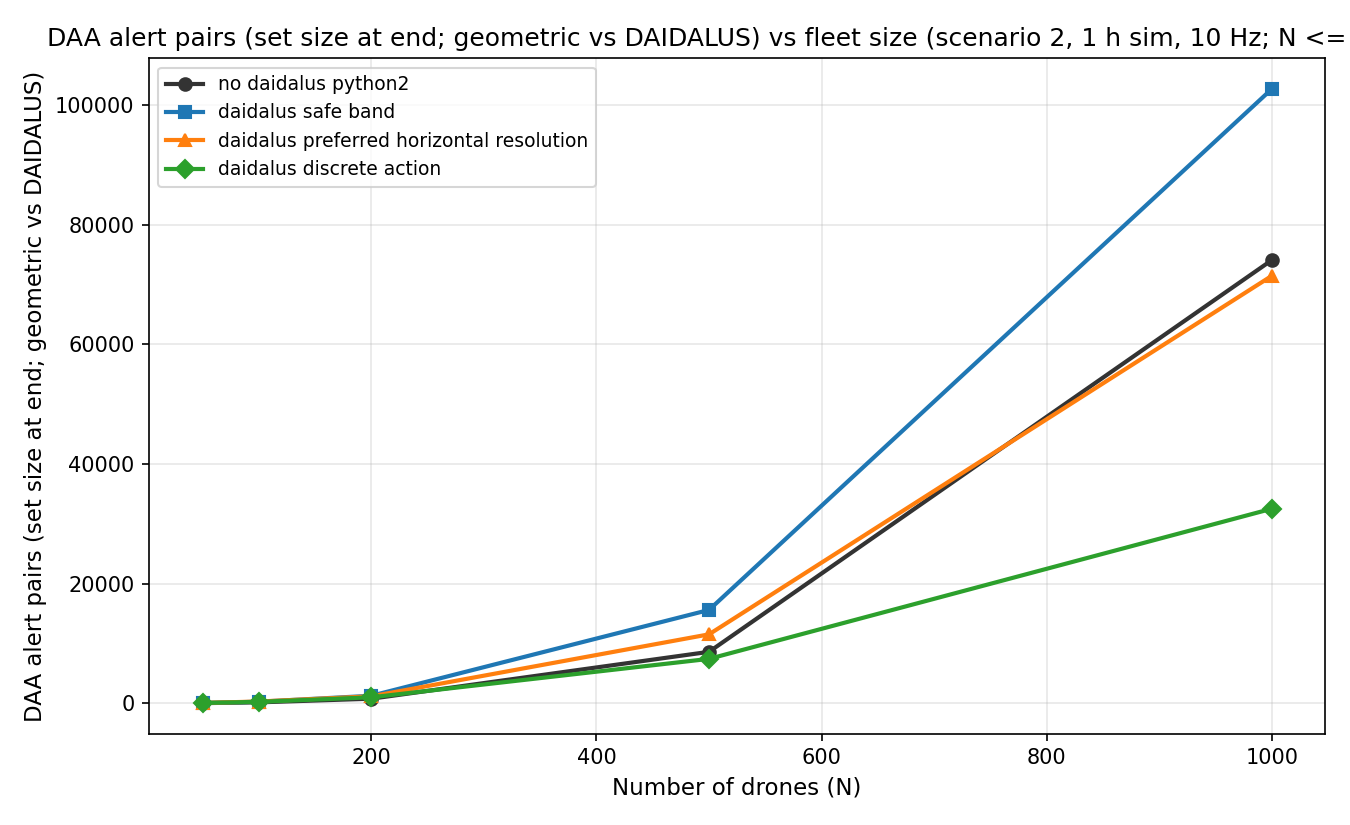
\includegraphics[width=\linewidth]{documentation/report_sections/figures/scen2_daidalus_sweep/fig_scen2_daa_alert_pairs_vs_n.png}}
\caption{DAA alert pair count vs fleet size.}
\label{fig:scen2_daa_pairs}
\end{figure}

\begin{figure}[htbp]
\centerline{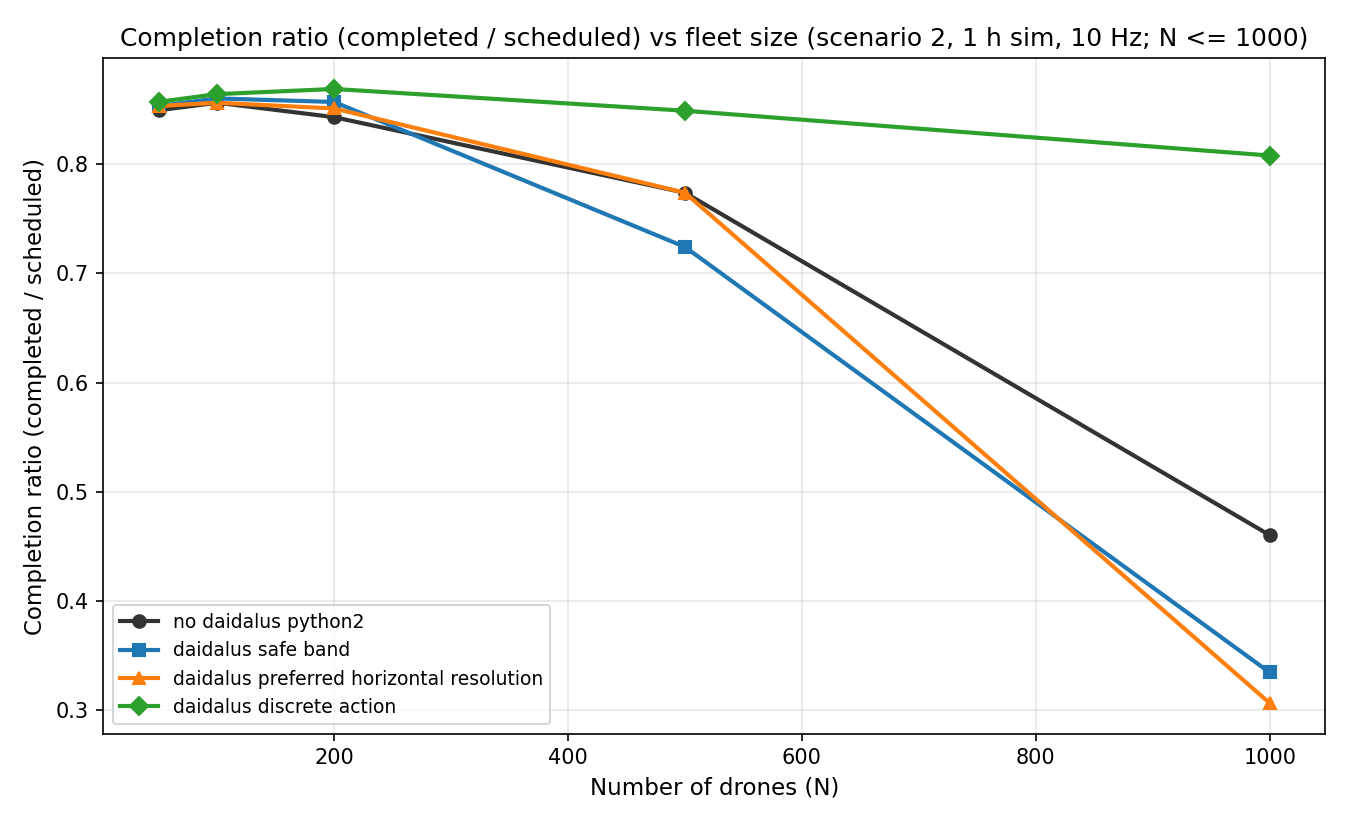
\includegraphics[width=\linewidth]{documentation/report_sections/figures/scen2_daidalus_sweep/fig_scen2_completion_ratio_vs_n.png}}
\caption{Completion ratio vs fleet size.}
\label{fig:scen2_completion}
\end{figure}

\begin{figure}[htbp]
\centerline{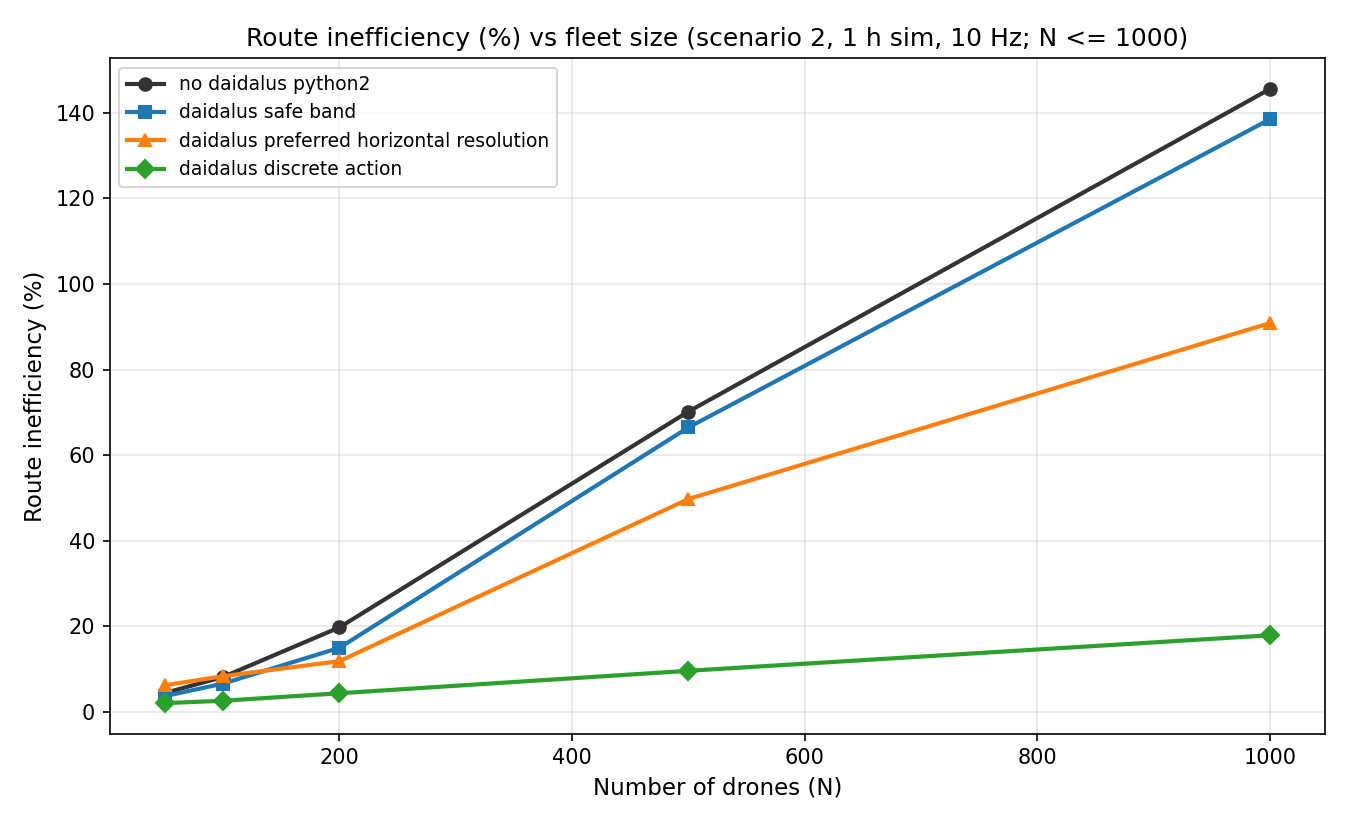
\includegraphics[width=\linewidth]{documentation/report_sections/figures/scen2_daidalus_sweep/fig_scen2_route_inefficiency_vs_n.png}}
\caption{Route inefficiency vs fleet size.}
\label{fig:scen2_ineff}
\end{figure}

\begin{figure}[htbp]
\centerline{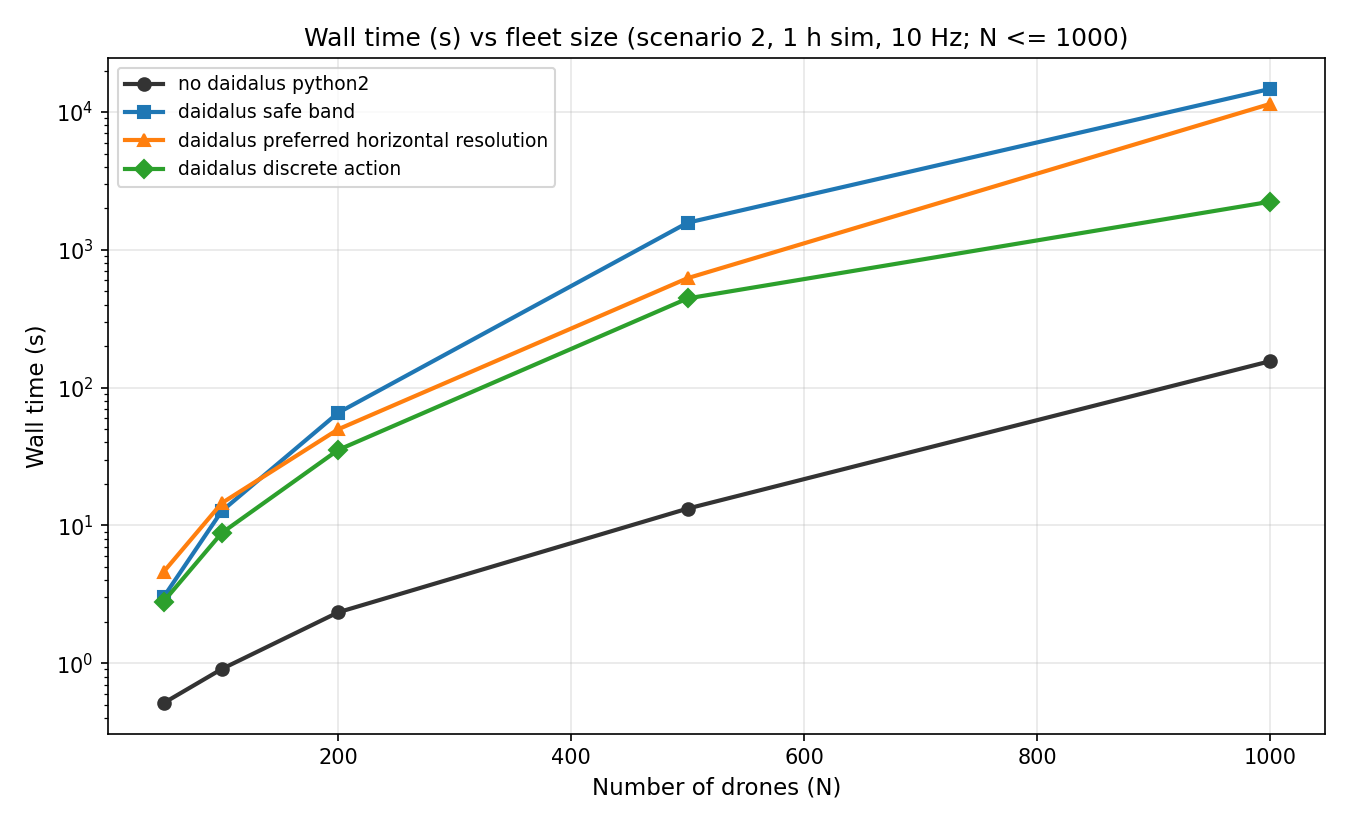
\includegraphics[width=\linewidth]{documentation/report_sections/figures/scen2_daidalus_sweep/fig_scen2_wall_seconds_vs_n.png}}
\caption{Wall-clock time vs fleet size.}
\label{fig:scen2_wall}
\end{figure}

\begin{figure}[htbp]
\centerline{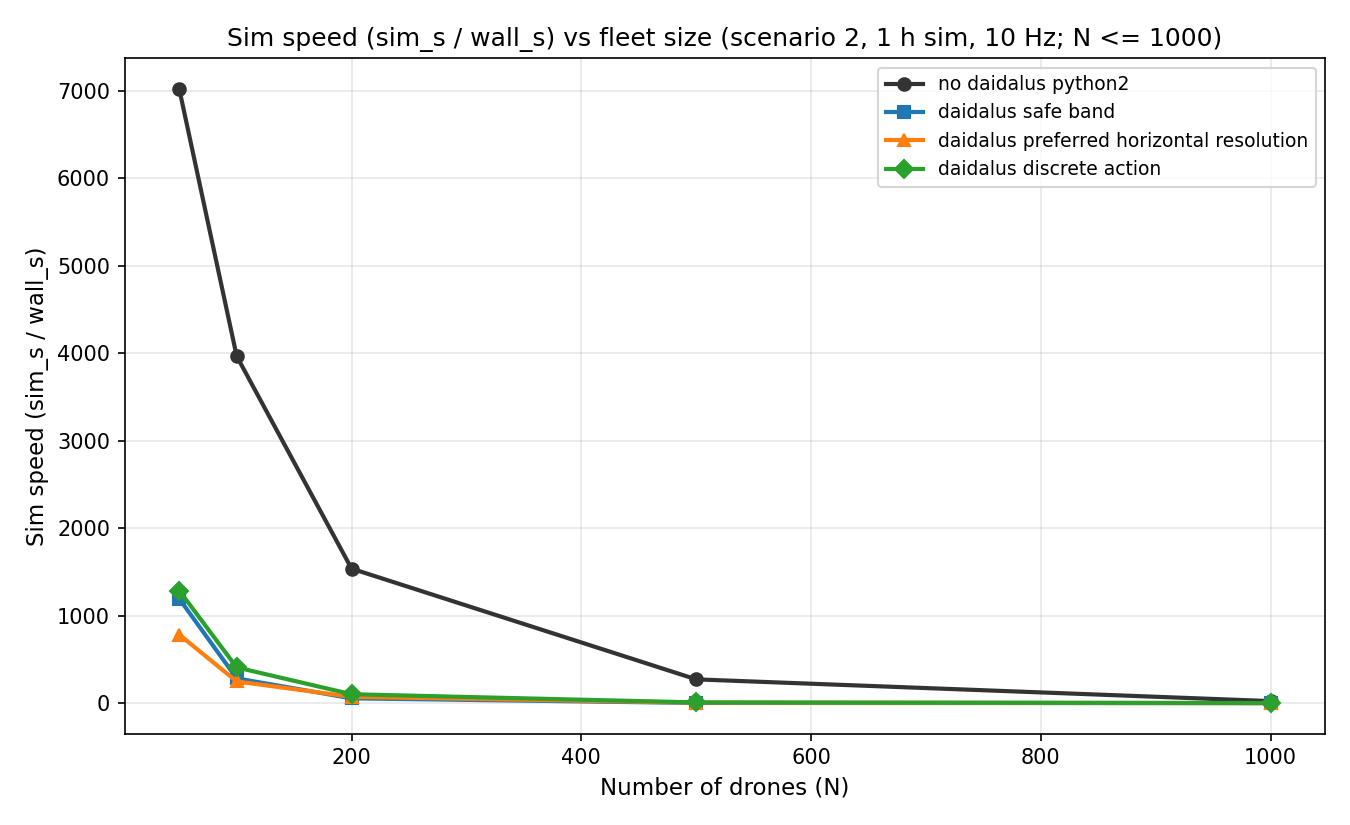
\includegraphics[width=\linewidth]{documentation/report_sections/figures/scen2_daidalus_sweep/fig_scen2_realtime_x_vs_n.png}}
\caption{Real-time factor (\texttt{sim\_seconds / wall\_seconds}) vs fleet size.}
\label{fig:scen2_realtime}
\end{figure}

\subsection{Discussion and implications}

\begin{itemize}
\item \textbf{Scalability breakpoint:} baseline (\texttt{no\_daidalus\_python2}) degrades strongly after $N=500$, and completion collapses further by $N=1000$.
\item \textbf{Action-mode sensitivity:} DAIDALUS behavior is dominated by action mode; \texttt{discrete\_action} is significantly more robust than \texttt{safe\_band} and \texttt{preferred\_horizontal\_resolution} in this scenario.
\item \textbf{Operational implication:} at high density, choice of tactical action mode can dominate both safety proxy metrics and mission throughput, not only trajectory quality.
\end{itemize}

\subsection{Caveats}

\begin{itemize}
\item \texttt{daa\_alert\_pairs} are mode-dependent (geometric shell in baseline vs DAIDALUS alerts in DAIDALUS modes); absolute values should be interpreted as trend indicators across $N$, not strict semantic equivalents.
\item This section reports one-seed results; confidence intervals require multi-seed repetition.
\end{itemize}
